\chapter{Background}
\label{ch:background}
This chapter will present the necessary background information for this thesis. Here, we define some basic terminology that will be used throughout this thesis.

\section{Code clone terminology}\label{sec:terminology}
% The sets are actually definitions, NOT PROPERTIES. This should be clearer.
Many studies present different definitions for code clone concepts. For this study, we mainly use the definitions from Bruntink et al. \cite{bruntink2005use}, Roy et al. \cite{roy2007survey} and Jiang et al. \cite{jiang2007deckard}. We created a summary of these concepts, which can be found in table \ref{tab:clone-terminology}.

\begin{table}[H]
\centering
\resizebox{\textwidth}{!}{%
\begin{tabular}{@{}lllll@{}}
\toprule
\rowcolor[HTML]{FFFFFF}
\textbf{Symbol} & \textbf{Meaning} & \textbf{Definition} & \textbf{Description} & \textbf{Properties} \\ \midrule
\rowcolor[HTML]{EFEFEF}
T & Token & - & \begin{tabular}[c]{@{}l@{}}Tokens are the basic lexical\\ building blocks of source code. \\ For this study, this is the smallest\\ relevant entity of a program.\end{tabular} & \begin{tabular}[c]{@{}l@{}}\textbf{Range (R):} The range this token\\spans.\\ \textbf{Category (C):} Identifier, Keyword,\\Literal, Separator, Operator,\\ Comment or Whitespace.\end{tabular} \\
\rowcolor[HTML]{FFFFFF}
N & Node \cite{jiang2007deckard} & Set of tokens. & \begin{tabular}[c]{@{}l@{}}A statement or declaration in a \\ codebase.\end{tabular} & \begin{tabular}[c]{@{}l@{}}\textbf{Range (R):} The range this node\\spans.\end{tabular} \\
\rowcolor[HTML]{EFEFEF}
I & \begin{tabular}[c]{@{}l@{}}Clone\\ instance \cite{bruntink2005use, roy2007survey}\end{tabular} & \begin{tabular}[c]{@{}l@{}}Set of cloned\\nodes.\end{tabular} & \begin{tabular}[c]{@{}l@{}}A code fragment that appears in\\ multiple locations.\end{tabular} & \begin{tabular}[c]{@{}l@{}}\textbf{File (F):} The file in which this\\clone instance is found.\end{tabular} \\
\rowcolor[HTML]{FFFFFF}
C & Clone class \cite{bruntink2005use, roy2007survey}& \begin{tabular}[c]{@{}l@{}}Set of clone\\instances.\end{tabular} & \begin{tabular}[c]{@{}l@{}}A set of similar code fragments in\\ different locations. Each of these\\code fragments is called a\\``clone instance''.\end{tabular} & - \\
\rowcolor[HTML]{EFEFEF}
S & \begin{tabular}[c]{@{}l@{}}Clone class\\ collection \cite{bruntink2005use}\end{tabular} & \begin{tabular}[c]{@{}l@{}}Set of clone\\classes.\end{tabular} & \begin{tabular}[c]{@{}l@{}}All clone classes that have been\\found for a certain software\\project.\end{tabular} & - \\
\rowcolor[HTML]{FFFFFF}
%R & Range & A part of a source code file. &  & \begin{tabular}[c]{@{}l@{}}\textbf{Begin line/column:} The line and column at \\ which the range starts.\\ \textbf{End line/column:} The line and column at\\ which the range end.\end{tabular} \\
 \bottomrule
\end{tabular}%
}
\caption{Clone related terminology and how it maps to the source code.}
\label{tab:clone-terminology}
\end{table}

A \textbf{range} denotes the line and column at which a code fragment starts and ends. In this study, we use the symbols given in this table in our formulas.

\subsection{Example}
This section gives an example to make the terminology of table \ref{tab:clone-terminology} more concrete. The code fragment in figure \ref{fig:cloneclasses} shows two clone classes. One of the clone classes consists of two clone instances and has three nodes per instance. The other clone instance has three clone instances and consists of two nodes per instance.

\begin{figure}[H]
\begin{parcolumns}{3}
\colchunk[1]{
\begin{javacode}
// File1.java
|\highlightDarkyellow|doA();
|\highlightDarkyellow|doB();
|\highlightYellow|doC();
\end{javacode}}
\colchunk[2]{
\begin{javacode}
// File2.java
|\highlightDarkyellow|doA();
|\highlightDarkyellow|doB();
|\highlightYellow|doC();
\end{javacode}}
\colchunk[3]{
\begin{javacode}
// File3.java
|\highlightYellow|doA();
|\highlightYellow|doB();
doD();
\end{javacode}}
\end{parcolumns}
\caption{Two clone classes: One clone class with three clone instances and one with two clone instances.}
\label{fig:cloneclasses}
\end{figure}

This example can be represented as a tree structure using the concepts from table \ref{tab:clone-terminology}. This tree structure is displayed in figure \ref{fig:terminologyexample}.

\begin{figure}[H]
  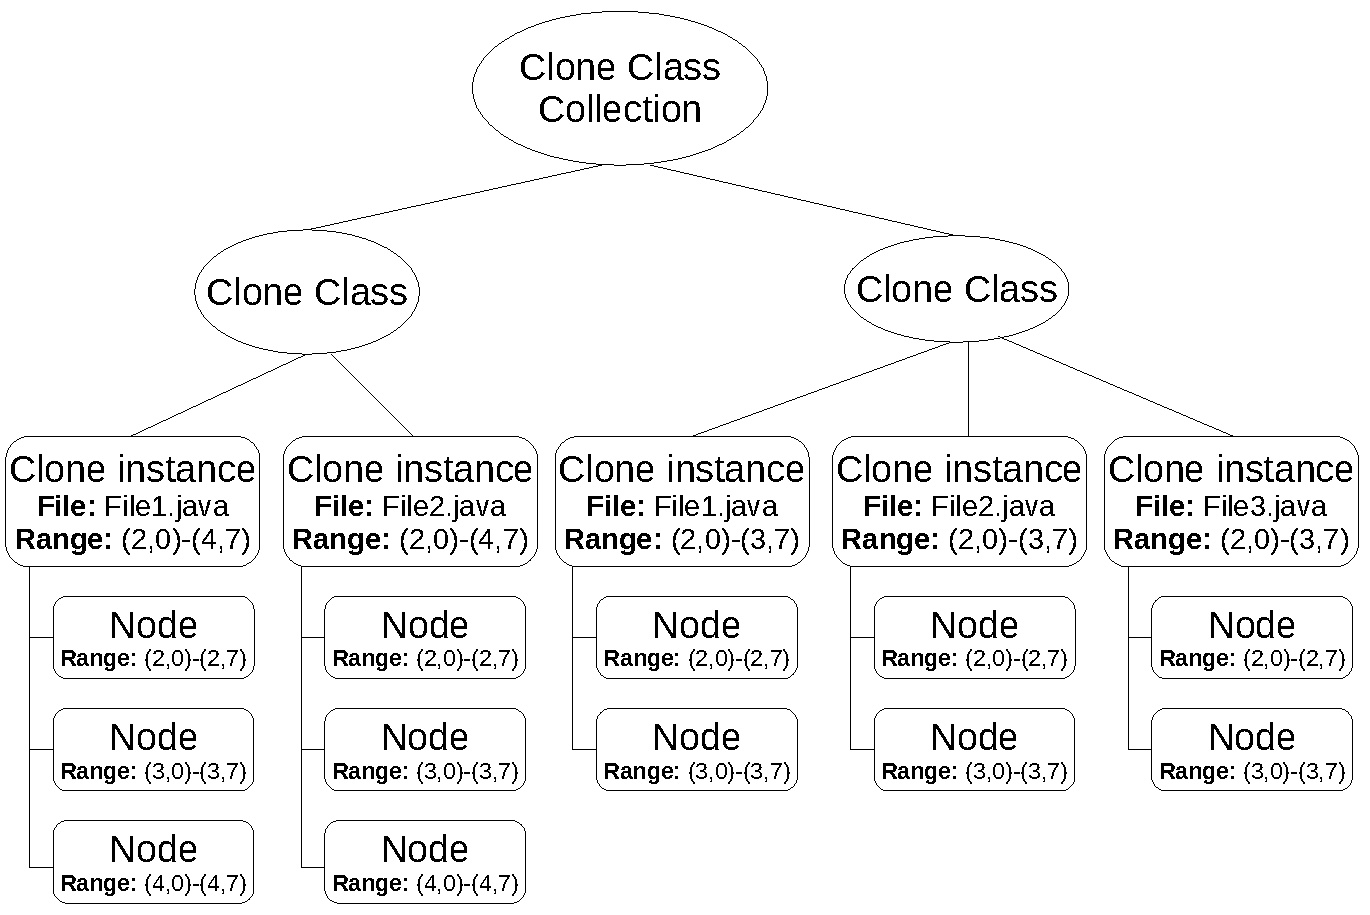
\includegraphics[width=1\columnwidth]{img/TerminologyExample}
  \caption{Representation of figure \ref{fig:cloneclasses} using the terminology introduced in table \ref{tab:clone-terminology}}
  \label{fig:terminologyexample}
\end{figure}

\section{Clone Types} \label{chap:backgroundclonetypes}
Duplication in code is found in many different forms. Most often duplicated code is the result of a programmer reusing previously written code \cite{haefliger2008code, baxter1998clone}. Sometimes this code is then adapted to fit the new context. To reason about these modifications, several clone types have been proposed. These clone types are described in Roy et al \cite{roy2007survey}:
\begin{displayquote}
\textbf{Type I:} Identical code fragments except for variations in whitespace (may be also variations in layout) and comments.\\
\textbf{Type II:} Structurally/syntactically identical fragments except for variations in identifiers, literals, types, layout and comments.\\
\textbf{Type III:} Copied fragments with further modifications. Statements can be changed, added or removed in addition to variations in identifiers, literals, types, layout and comments.\\
\textbf{Type IV:} Two or more code fragments that perform the same computation but implemented through different syntactic variants.
\end{displayquote}
A higher type of clone means that it's harder to detect and refactor. There are many studies that adopt these clone types, analyzing them further and writing detection techniques for them \cite{sajnani2016sourcerercc, kodhai2010detection, van2019novel}.

\subsection{Type 4 clones}
For this study we have chosen to take type 4 clones out of the scope, because they are both hard to detect and hard to refactor. A study by Kodhai et al \cite{kodhai2013method} looks into the distribution of the different types of clones in several open source systems (see table 6 of his study). It becomes apparent that type 4 clones exist way less in source code than all of the other types of clones. For instance, for the J2sdk-swing system he finds 8115 type 1 clones, 8205 type 2 clones, 11209 type 3 clones and only 30 type 4 clones. Because of that, we can conclude that type 4 clones are relatively less relevant to study.

\section{Refactoring methods}
Martin Fowler recently released the second edition of his Refactoring book \cite{fowler2018refactoring}. In this book he exclaims that \textit{``if you see the same code structure in more than one place, you can be sure that your program will be better if you find a way to unify them''} \cite{fowler1999refactoring, fowler2018refactoring}. He describes several methods to deal with duplication, dependent on the context of the clone. In this section we describe the methods which we use in this study.

\subsection{Extract Method}
The main method for dealing with duplication in source code, as described by Martin Fowler, is to extract the duplication to a common place. This refactoring method is called ``Extract Method''. Several studies have already concluded that most duplication in source code is found in the body of methods \cite{lozano2007evaluating, white2016deep, bergman2004ethnographic}. Method extraction can move matching functionality in method bodies to a common place, namely a new method. An example of this procedure is displayed in figure \cite{fig:extractmethod}.

\begin{figure}[H]
\begin{parcolumns}{2}
\colchunk[1]{
\begin{javacode}
// Original
public void doStuff(){
|\highlightYellow|  doA();
|\highlightYellow|  doB();
  doC();
|\highlightYellow|  doA();
|\highlightYellow|  doB();
}
\end{javacode}}
\colchunk[2]{
\begin{javacode}
// Refactored
public void doStuff(){
|\highlightYellow|  doAandB();
  doC();
|\highlightYellow|  doAandB();
}

public void doAandB(){
  doA();
  doB();
}
\end{javacode}}
\end{parcolumns}
\caption{Refactoring a clone class through method extraction.}
\label{fig:extractmethod}
\end{figure}

\subsection{Move method}
In the example of the previous section, both duplicated parts are in the same method. However, a study by Fontana et al. \cite{fontana2015duplicated} shows that this is most often not the case. Based on the relation between clone instances, the extracted method must be moved to be accessible by all locations of the clone instances. This might require different techniques.

\subsubsection{Pull up method}
A refactoring technique to move a method up in its inheritance structure is called ``Pull up method'' \cite{fowler2018refactoring}. This way, if cloned methods are related in any way through inheritance, they can be called by both classes by placing the method in a class they both have in common. This way its possible to refactor both fully cloned methods (by just pulling up the method) and partially cloned methods (by first performing method extraction and then pulling up the refactored method).

\subsubsection{Create class abstraction based on implicit relations}
Duplication in source code is an implicit relation between fragments of source code. If two classes have many of these implicit relations, then the implementation should be refactored to make this relation explicit. If the classes do not yet have a parent/super class, a parent class can be created and the common functionality can be placed in this newly created class. This makes the relation between these classes explicit and reduces duplication.

\subsubsection{Providing default implementations for common functionality}
Looking specifically at the Java programming language, recent versions of Java introduce a new method of reducing duplication through refactoring. Java has the concept of \textit{interfaces} as an abstract type that is used to specify a behavior that classes must implement. Since Java version 8, Java also supports default implementations to be provided in interfaces \cite{mohnen2002interfaces}. This gives an opportunity to make the relation between classes explicit and reduce duplication. It can be used in instances where creating a new parent class for duplicated classes is undesirable.

\subsection{Clone refactoring in relationship to its context}
How to refactor clones is highly dependent on their context. Method-level clones can be extracted to a method \cite{kodhai2013method} if all occurrences of the clone reside in the same class. If a method level clone is duplicated among classes in the same inheritance structure, we might need to pull-up a method in the inheritance structure. If instances of a method level clone are not in the same inheritance structure, we might need to either make a static method or create an inheritance structure ourselves. So not only a single instance of a clone has a context, but also the relationship between individual instances in a clone class. This is highly relevant to the way in which the clone has to be refactored.

\section{Internal and external classes}
In this study we differentiate between \textit{internal} and \textit{external} classes. Classes are the components of a software system that contain its functionality. When analyzing a software system, \textit{Internal classes} are classes that belong to this software system specifically, and its source code is included in the project.

\textit{External classes} are classes that a software system uses, but do not belong to this specific software system. Typically, the source code of external classes are not included in the source code of the project. Most often these external dependencies are referenced in a file that its build automation system uses to fetch a projects' dependencies.

Regarding refactoring, a software system can often not change the source code of its dependencies. This can sometimes be a burden, when an external dependency does not use proper abstractions that are required by a software system. Because of that, in this study, we differentiate between internal and external classes to see what impact they have on the refactoring process.\todo{you don't consider external right?}

\subsection{Maven}
For this study we perform a shallow analysis on external dependencies, in order to derive more context for internally used concepts. As these external dependencies are most often not included in a software systems' source code, we must first use the projects' build automation system to gather the dependencies. To limit the scope of this process, we decided to focus on only the \textit{Maven} build automation system.

Maven is a build automation tool, mainly used with the Java programming language. Maven has a simple ecosystem to configure and fetch the binaries and source code of all software projects a given codebase is dependent on. Maven can also be used to run tests for the systems and to package the project as an executable file.

\section{(Object-Oriented) Programming Languages}
In this section we describe the relevant parts of the programming languages we research and experiment on.

\subsection{AST} \label{sec:astbackground}
An Abstract Syntax Tree (AST) is a tree consisting of an hierarchical representation of the source code of a program. Detecting code clones on the AST of a program allows for a deeper understanding of the concepts that are being analyzed. Having an AST, we know how concepts in the code are related. This helps to determine in what classes and methods cloned code is found.

Having access to a programs' AST also helps in the process of refactoring. Moving AST nodes rather than textual modifications reduces error margins because the tree structure stays intact.

The AST consists of nodes of the following types (examples are for Java):
\begin{itemize}
  \item \textbf{Declarations}: Method-declaration, class-declaration, etc.
  \item \textbf{Statements}: If-statement, switch-statement, expression-statement, etc.
  \item \textbf{Expressions}: Variables, literals, method calls, variable assignments, etc.
  \item \textbf{Types}: Primitives, reference types, void, etc.
  \item \textbf{Clauses}: Catch-clause, else-clause, etc.
\end{itemize}

\subsection{Inheritance}
Object-Oriented programming languages use inheritance to model real-world relations between data concepts. Inheritance allows an object to inherit all functionality from another object. For instance, a ``Car'' object would inherit functionality and data from generalized concepts, such as ``Vehicle''. Using inheritance it is possible to reduce duplication, as multiple objects can inherit common functionality.

When looking at the inheritance structure of a program, we can get a deeper understanding of a programs' architecture. The use of inheritance to group common functionality and data is called ``Abstraction''. Duplication in source code can be a result of an inadequate use of abstraction. Because of that, refactoring code clones might require to create such abstractions of common functionality.

\subsection{Code Quality}
Different programming languages have different ways to measure code quality. For object-oriented programming languages this largely comes in the form of code smells (patterns that should be avoided) and design patterns (patterns which may improve code design and comprehensibility when used correctly).

\subsubsection{Code Smells}
Code smells are patterns in code that should be avoided, because they have a negative effect on system design. Duplicate code is, among many others, one example of a code smell. Having many code smells present in source code can significantly increase maintainence costs of the source code or even render a software system unmaintainable. This increases technical debt: a debt present in the system the will have to be repaid at a later point of time. Such technical debt often comes at the expense of developing new features, fixing bugs and other aspects surrounding a programs functional behaviour.

\subsubsection{Design Patterns}
Most code smells have design patterns that can be used to mitigate the smell. For instance, duplicate code can be mitigated by using appropriate abstractions or refactoring duplicate code to a common place. Design patterns differ from refactoring methods in the sense that they are more about an architectural pattern rather than a certain kind of code modification.

\subsubsection{Maintainability Metrics}
Maintainability metrics are features of source code by which an indication of the maintainability of the source code can be measured. Heitlager at al. \cite{heitlager2007practical} propose a maintainability model that categorize the results of metrics into different ``score'' categories. For instance, with duplication, if 0-3\% of the project is duplicated, the project will get the highest score on a scale of 1 to 5 (only integers, no floating point numbers). Such a maintainability model is intuitive for measuring the quality of a software system, especially large software systems with a lot of source code to base the metrics on. However, this maintainability model \cite{heitlager2007practical} lacks in measuring fine-grained changes: most small changes will not fall into a different category. Because of that, this model is less suitable for measuring the impact of single refactorings.

\subsection{Java}
We run all our experiments on projects written in Java. Because of that, we get some information that is specific to Java systems. Additionally, we perform automated refactorings on Java systems, which requires the use of Java language concepts. These are explained in this section. Many of these concepts also exist in other programming languages, but often not in all.

\subsubsection{Interfaces}
Java uses the concept of interfaces to loosely couple a specification and its implementation. Interfaces are specifications about what a (group of) objects do. Often, methods don't need an entire object, but just use a few properties of it. Because of that, Java recommends to program to an interface rather than an implementation. This means that we should use abstractions of expected functionality rather than complete implementations of functionality. This can make switching implementations at a later point in time easier.

Often, duplication is the result of an inappropriate use of abstractions. Two methods might describe operations on types following the same contract, but because of a lack of abstraction the programmer may choose to clone such methods. This will result in duplicated methods with minor modifications to match a different implementation. Such duplicates can be mitigated by using proper abstractions, of which one option is to program methods against interfaces (contracts of expected functionality) rather than their full implementations.

\subsubsection{Packages}
Packages (sometimes called ``modules'' in other programming languages) are hierarchical groupings of related concepts. For instance, all UI logic in an application might go into the ``ui'' package. The ``ui'' package can have a subpackage named ``keyhandling'' for all keyhandling operations. These packages contain package-level declarations, like classes and interfaces. Names of class-level declarations must be unique within the package. However, duplicate declaration names may exists in subpackages and parent packages.

In Java, all declarations used from outside the package a declaration is in, must be \textit{imported}. Importing a declaration from outside the current package goes by the fully qualified identifier (FQI) of the declaration. The FQI of a declaration gives an unique identifier for a symbol in a codebase. For instance, if our ``keyhandling'' package would contain a ``KeyHandler'' class, its fully qualified identifier would be ``ui.keyhandling.KeyHandler''.

\subsubsection{Visibility}
In Java, we can protect declarations from being used in scopes in which they are supposed to be used. If a method should only be used within the class itself, we can give it a ``private'' visibility. If a method is to be used by its children in its inheritance hierarchy, we can set its visibility to ``protected''. If a method is supposed to be part of the public contract of an object, we can set it to ``public'' visibility. Alternatively, there is ``package'' visibility, for declarations that should only be referenced within the same package. This allows control over what parts of an application should be able to access what declarations.
